\graphicspath{{Billeder/}}
\chapter{Test}
\section{Unit tests}
Link til Jenkins - Unit tests: \url{http://ci3.ase.au.dk:8080/job/TeamTyveATMUnitTest/} \newline 

Der er valgt ikke at teste ConsoleLogger.cs, da denne skriver direkte til konsollen, og det er ikke muligt at erstatte statiske metoder. Det vil derfor ikke være muligt at teste om Console.WriteLine() udskriver det korrekte. 

Ydermere er der få andre klasser der ikke er blevet unit testet. Dette skyldes at disse klasser for eksempel kun indeholder entiteter, eller ikke har nogen logik i sig. Derfor vil det ikke give nogen videre værdi at teste disse.

\section{Integrationstests}
Link til Jenkins - Integrationstests: \url{http://ci3.ase.au.dk:8080/job/TeamTyveATMIntegrationTest/} \newline

\textbf{Dependency Tree} \newline
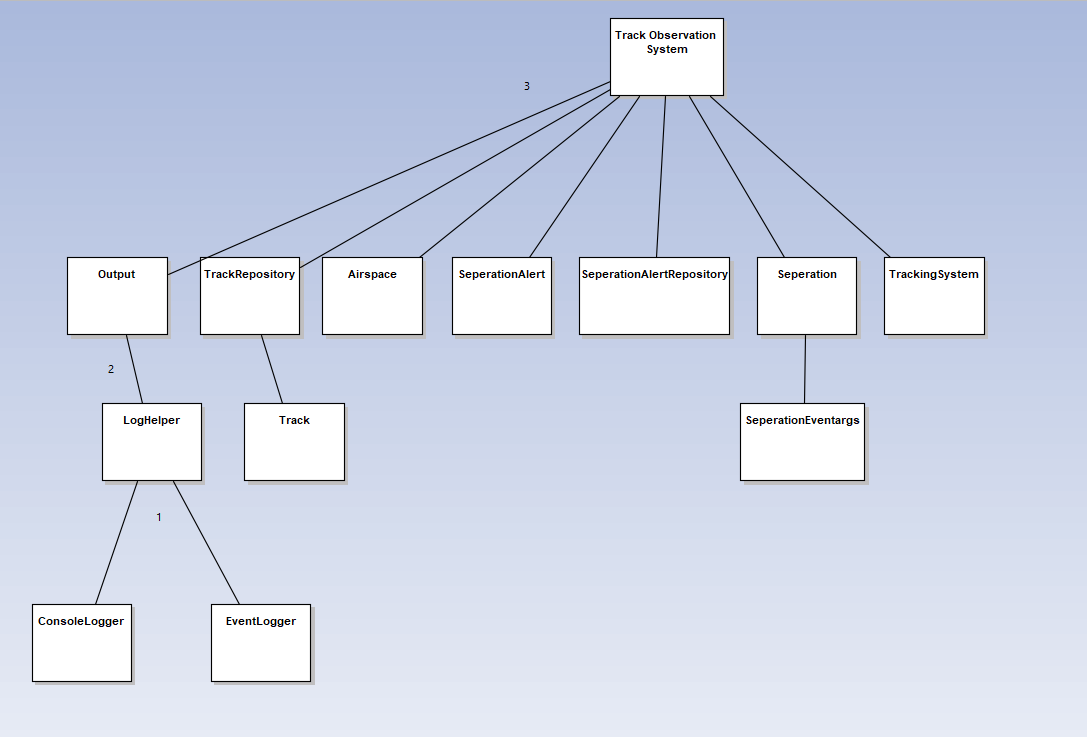
\includegraphics[scale=0.65]{dependencyTree.PNG} \newline
Ovenstående ses dependency-tree for systemet. Der er i alt tre steps, hvor der er valgt at teste det nederste lag først, og derfra bevæge sig op. Altså er bottom up valgt som integrationsstrategi \newline

Denne strategi er valgt grundet at der derved er færre komponenter der skal stubbes, samt at det har virket intuitivt at bruge denne strategi.

Generelt set går bottom up testing ud på at starte fra bunden i det tilhørende dependency tree. De nederste klasser, og derved de klasser der afhænger af mindst vil blive testet først. Hvorfra der hierakisk vil blive testet op igennem træet, indtil alle forbindelser imellem klasserne er blevet tests. Der vil altså blive testet fra submodulerne til hovedmodul(erne).
En af fordelene ved bottom up strategien er at det kan eliminere behovet for anvendelse af stubbe i og med at der ikke er nogle højerestående dependencies at tage højde for. Dog er en af ulemperne ved strategien, at man får testet den overordnet funktionalitet sent i processen, og der derfor er risiko for at man skal lave noget af systemet om, senere end nødvendigt. \newline

\textbf{Integrationsplan} \newline
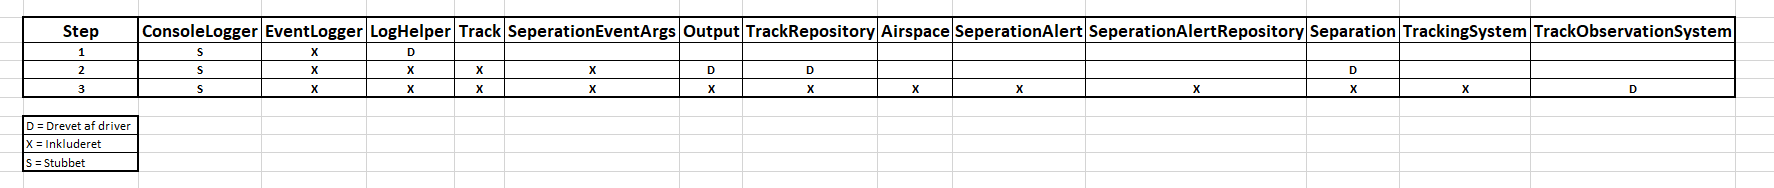
\includegraphics{plan.PNG} \newline
Integrationsplanen viser hvordan de forskellige klasser er inkluderet eller stubbet under de forskellige steps i integrationstesten. Integrationsplanen er lavet med udgangspunkt i dependency træet.


